\begin{figure}[!h]
	\centering
	\subbottom[Zurich, with beam search\label{fig:withbszh}]{
		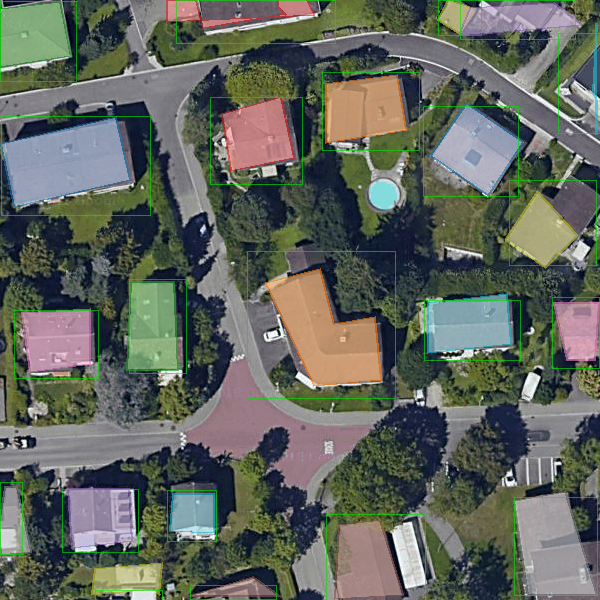
\includegraphics[width=\figfigfigfig\textwidth]{4-10-0.png}
		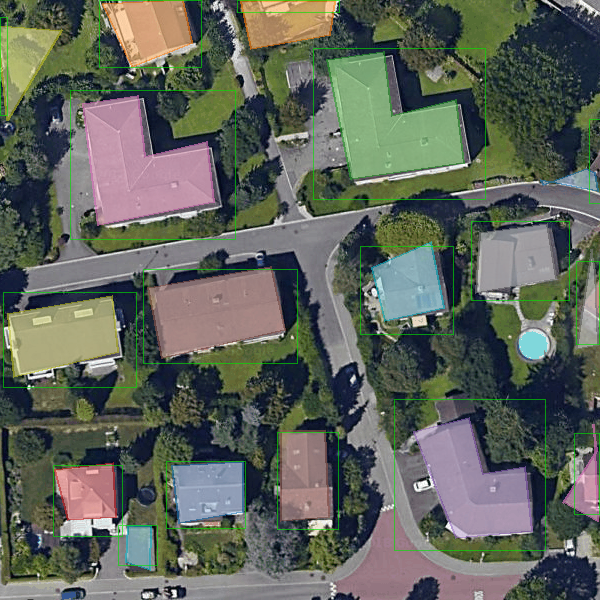
\includegraphics[width=\figfigfigfig\textwidth]{4-10-1.png}
		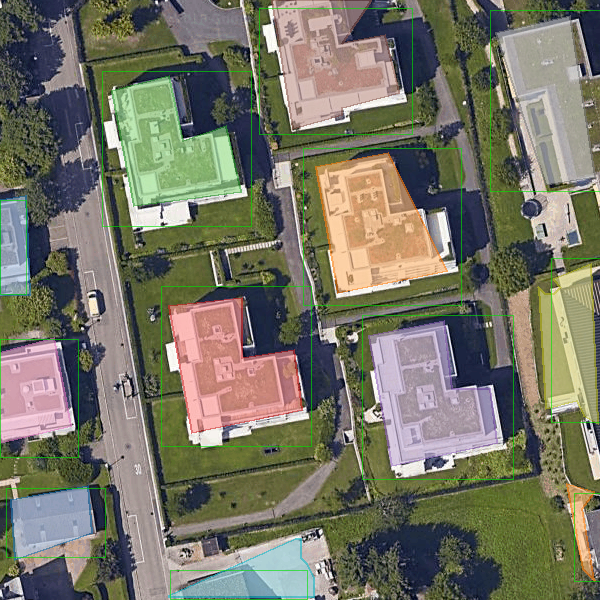
\includegraphics[width=\figfigfigfig\textwidth]{4-10-2.png}
		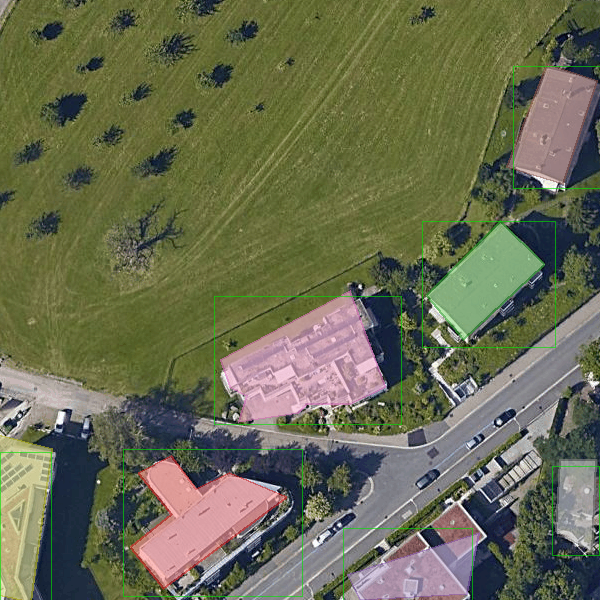
\includegraphics[width=\figfigfigfig\textwidth]{4-10-3.png}
	}
	\subbottom[Zurich, without beam search\label{fig:withoutbszh}]{
		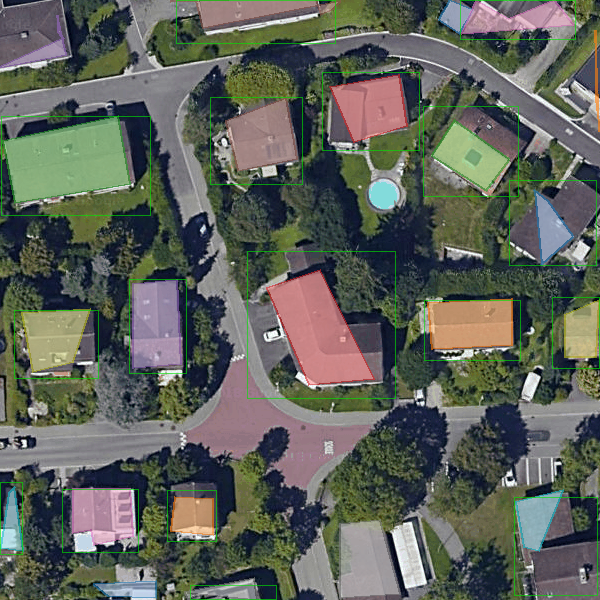
\includegraphics[width=\figfigfigfig\textwidth]{4-10-4.png}
		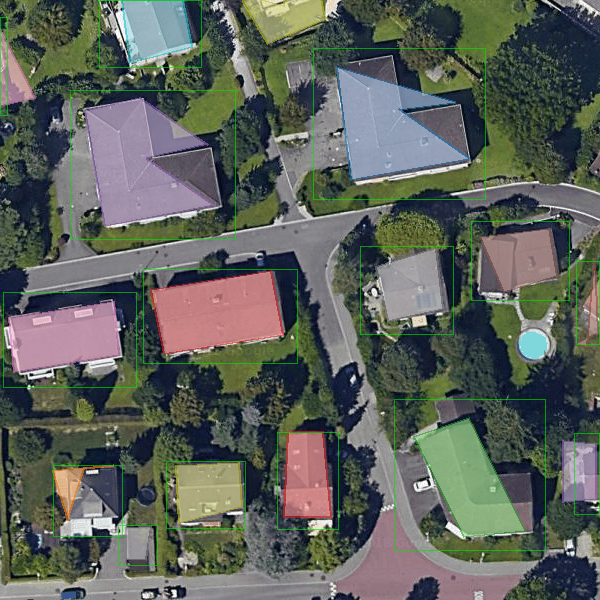
\includegraphics[width=\figfigfigfig\textwidth]{4-10-5.png}
		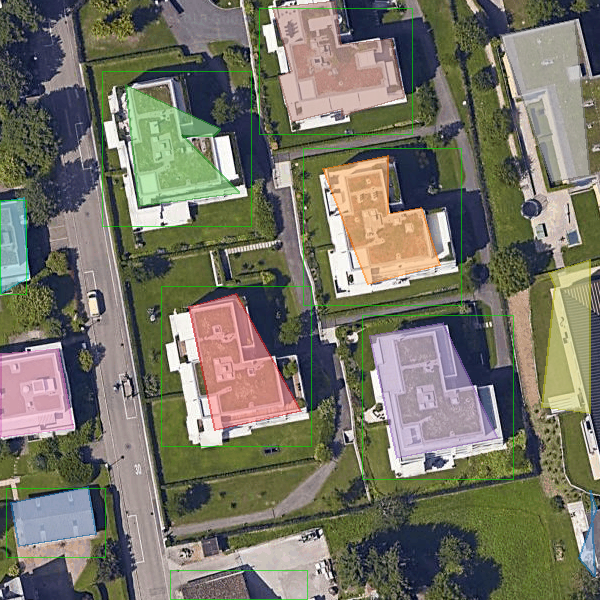
\includegraphics[width=\figfigfigfig\textwidth]{4-10-6.png}
		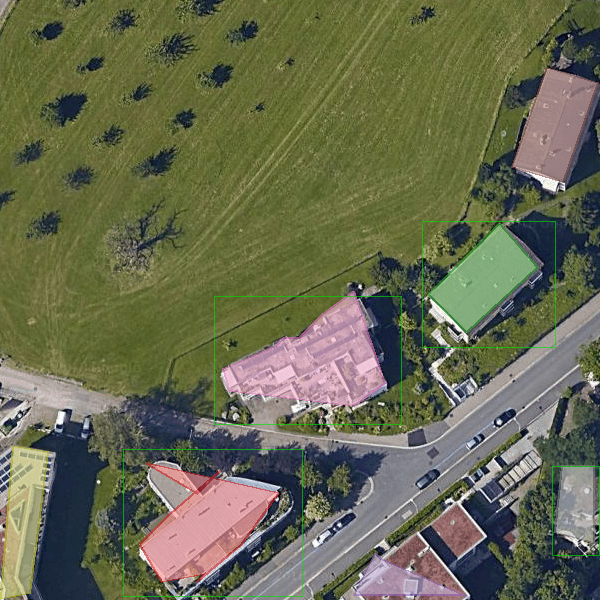
\includegraphics[width=\figfigfigfig\textwidth]{4-10-7.png}
	}
	\subbottom[Chicago, with beam search\label{fig:withbsch}]{
		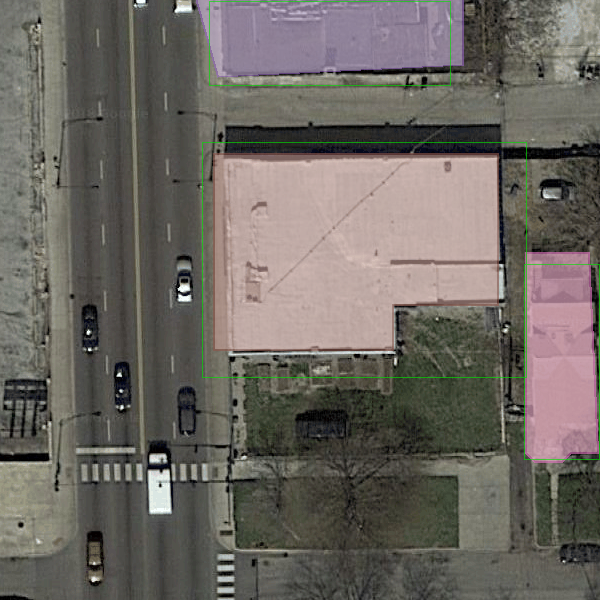
\includegraphics[width=\figfigfigfig\textwidth]{4-11-0.png}
		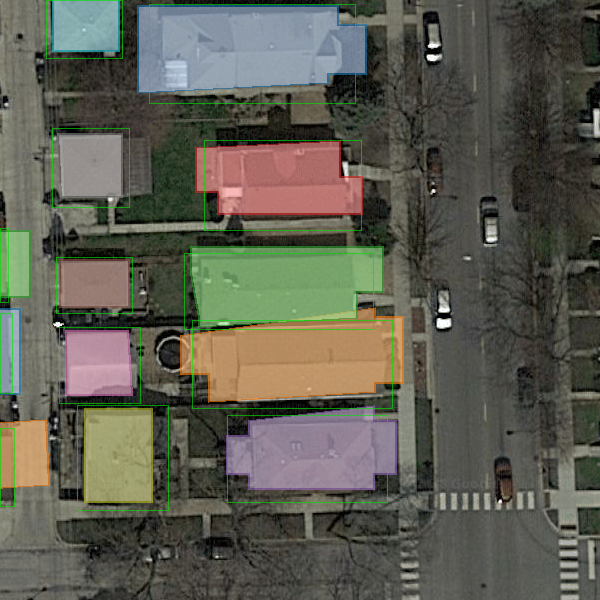
\includegraphics[width=\figfigfigfig\textwidth]{4-11-1.png}
		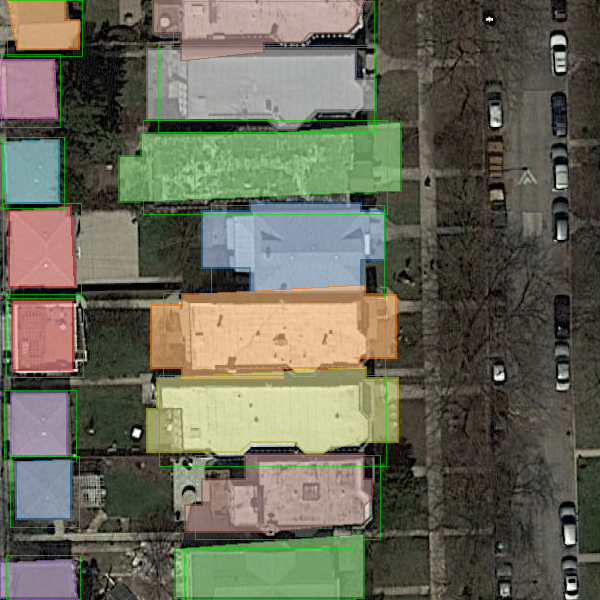
\includegraphics[width=\figfigfigfig\textwidth]{4-11-2.png}
		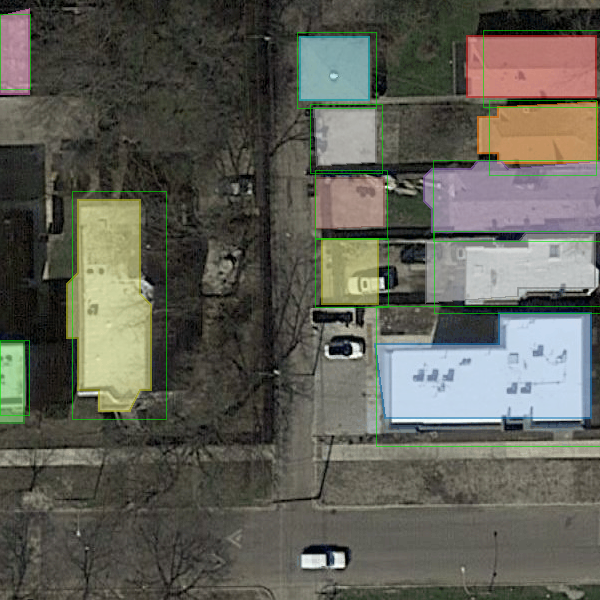
\includegraphics[width=\figfigfigfig\textwidth]{4-11-3.png}
	}
	\subbottom[Chicago, without beam search\label{fig:withoutbsch}]{
		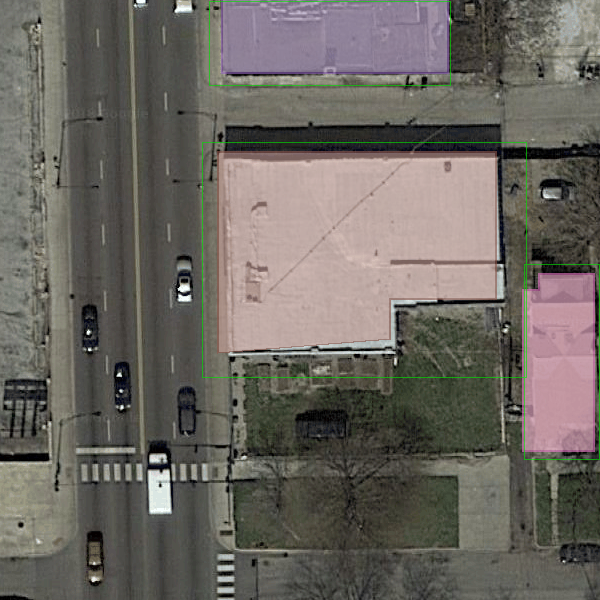
\includegraphics[width=\figfigfigfig\textwidth]{4-11-4.png}
		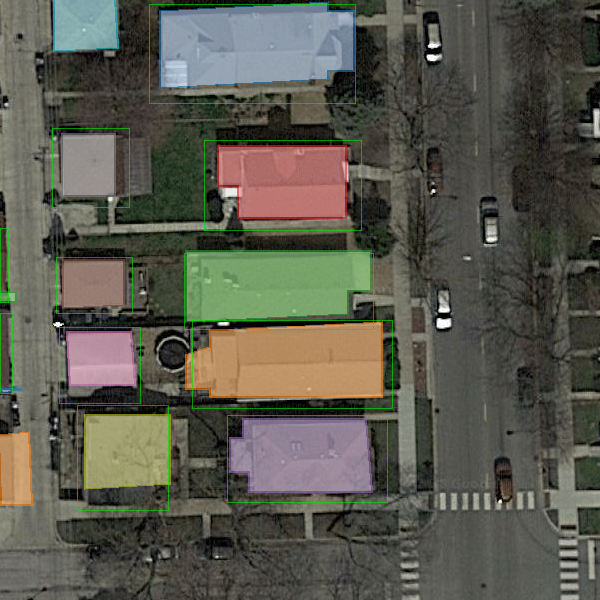
\includegraphics[width=\figfigfigfig\textwidth]{4-11-5.png}
		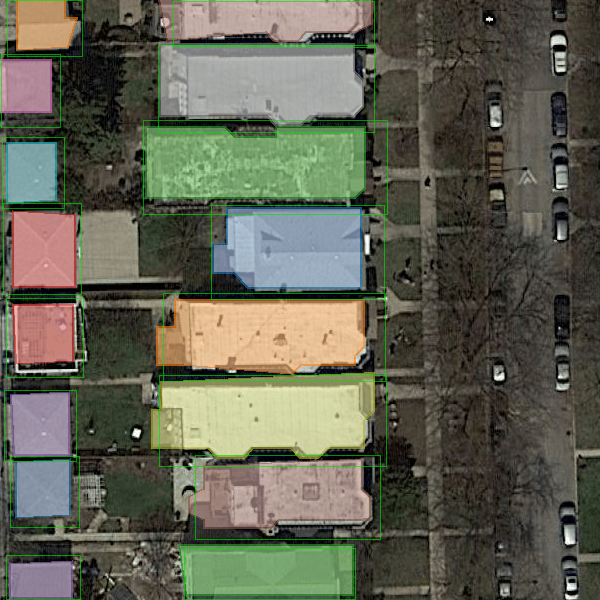
\includegraphics[width=\figfigfigfig\textwidth]{4-11-6.png}
		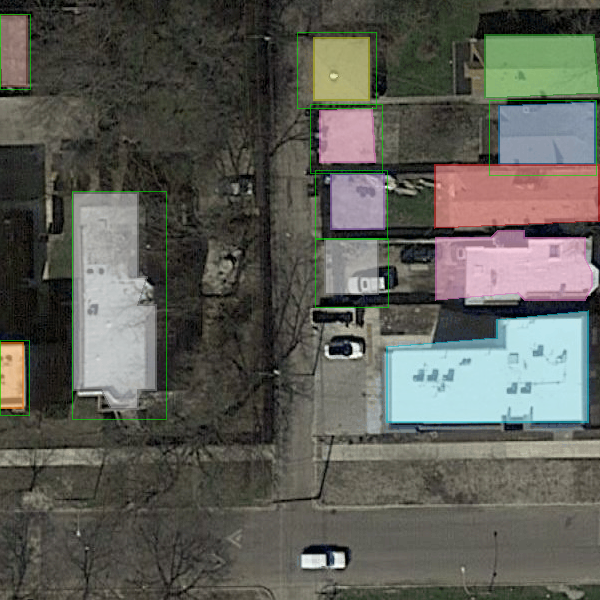
\includegraphics[width=\figfigfigfig\textwidth]{4-11-7.png}
	}
    \caption[Comparison of results in Zurich and Chicago in terms of beam search]{Comparison of results in Zurich and Chicago in terms of beam search.}
	\label{fig:compbs}
\end{figure}
